
\section{Problem definition}

In a graph, an irreversible conversion process refers to the spreading of a characteristic through the graph, later referred here as an infection, where we have information on the stage of this process at each instant of time.  
Given a graph $G = (V, E)$, this process will be analyzed as a sequence of binary labels that determines if a particular vertex in that instant of time is active or inactive
\begin{equation}
c_{t}: V(G) \rightarrow \{0,1\}
\end{equation}
\begin{equation}
C = (c_{0}, c_{1} \dots )= (c_{t \in \mathbb{N}})
\end{equation}
The way the characteristic spreads through the graph is controlled by a threshold function $ f $, or later refereed here as the vertices' resistance, is defined as:
\begin{equation}
f: V (G) \rightarrow \mathbb{Z}^+.
\end{equation}

Now, given an initial graph where each vertex has a resistance to the "infection", if we have a initial subset of vertices in this graph that will start carrying the infection, an uninfected vertex will be infected if the total of its already infected neighbors surpasses the vertex's resistance. More formaly, given a $ G $ graph and a threshold function $ f $, the process begins with an initial binary labeling $ c_{0} $ of the vertices, while the rest of the labels are iteratively defined so that $\forall t \in \mathbb{Z}^+, t > 0$ e  $\forall u \in V(G)$
\begin{equation}
c_{t}(u) = 1 \iff  c_{t-1}(u) = 1 \lor \sum_{v \in N_{G}(u)} c_{t-1}(v)  \geq f(u). 
\end{equation}

 %The main problem in this dissertation consists of, given an initial instance of graph and resistance function, what is the least number of vertices that need to be initially infected so to assure all the graph eventually will be completely infected. 


Figure \ref{fig: graph1} shows an example of an irreversible conversion process over time, with two vertices being initially infected.

\begin{figure}
  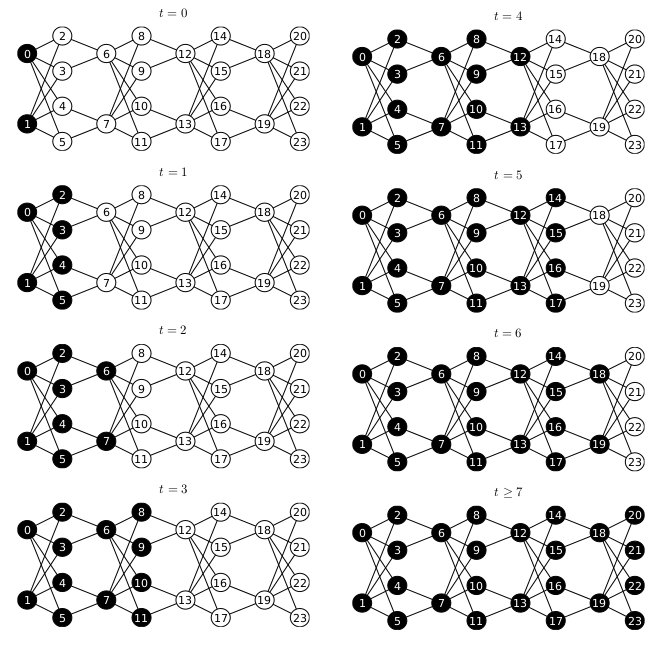
\includegraphics [width = \linewidth]{img/Figure3-1.png}
  \caption{Irreversible conversion process at different time points t for graph
of order 24, starting the process with convergent set and threshold function defined as $ f: V (G) \rightarrow {2}$. Source: \cite{amaral2015}}
  \label{fig: graph1}
\end{figure}

A convergent set is a label $ c_{0} $ which determines a certain sequence of labels $ c_ t$where

\begin{equation} 
\exists\ t_{s} \mid  v \in V(G) : c_{t_{s}}(v) = 1,
\end{equation}
and this set is denoted as
\begin{equation} 
\mathcal{C} = \{v \in V(G) : c_{0}(v) = 1\}
\end{equation}

  It follows from the definition that a trivial convergent set is $ V (G) $ itself. The minimum convergent set problem, or target set selection problem, is to find a convergent set as small as possible.

Given a constant threshold function $ f: V (G) \rightarrow \{k \}$ constant, \cite{centeno2011} has shown that this problem is NP-complete for any $ k \geq 2 $.

\section{Initial Formulation}

From these definitions, let the binary variable $ c_{t} (v) $ be the label of a vertex $ v $ in the instant $ t $ in our integer model.  $ c_{t} (v) = 1 $ will indicate if the vertex is infected (or active) and $ c_{t} (v) = 0 $ if not.

With this representation, it is evident that we want to minimize the number of infected tags at time 0, the initial infected vertices:
\begin{center}
\begin{equation}
min \sum_{v \in V} c_{0}(v)
\end{equation}
\end{center}


Also, for a workable solution to the problem, it is necessary to ensure that
\begin{center}
\begin{equation}
\begin{split} 
c_{t}(v) = 1 \iff c_{t-1}(v) = 1  \lor	 \sum_{\substack{ u \in \mathcal{N}_{G}(v) }} c_{t-1}(u) \geq f(v) \\ \\
\forall t \in 1, \ldots, |V|-1, v \in V 
\end{split}
\end{equation}
\end{center} 
which means that a vertex v has the label 1 (signiling it is infected) at a given instant t, then one of the following must be true:
\begin{itemize}
\item This vertex in the previous time instant was 1; or
\item In the previous time instant the number of infected neighbors of v surpassed f(v), threshold function of v.
\end{itemize}


Below, we separate the previous implication in multiple parts and translate them into linear restrictions that will have the same meaning in the model.

To represent the restriction that a label is infected at instant $ t $ implies that it is at the instant $ t + 1 $, that is
\begin{equation}
c_{t-1}(v) \implies c_{t}(v)
\end{equation}
we will use the constraint
\begin{equation}
c_{t-1}(v) \leq c_{t}(v).
\end{equation}
And the other part of our implication 
\begin{equation}
\sum_{\substack{ u \in \mathcal{N}_{G}(v) }} c_{t-1}(u) \geq f(v)  \implies c_{t}(v)
\end{equation}
can be described as
\begin{equation}
\sum_{u \in \mathcal{N}_{G}(v)}c_{t-1}(u) - f(v) + 1 \leq |V|c_{t}(v)  
\end{equation}
Now to show the implication back, that is
\begin{equation}
c_{t}(v) = 1 \\ \implies c_{t-1}(v) = 1 \lor	 \sum_{\substack{ u \in \mathcal{N}_{G}(v) }} c_{t-1}(u) \geq f(v)  
\end{equation}
or its contrapositive
\begin{equation}
c_{t-1}(v) == 0  \land \sum_{\substack{ u \in \mathcal{N}_{G}(v) }} c_{t-1}(u) < f(v) \\ \implies c_{t}(v) = 0  
\end{equation}
we have the following representation
\begin{equation}
\sum_{u \in N_{G}(v)}c_{t-1}(u) + f(v) \cdot c_{t-1}(v) \geq f(v) \cdot c_{t}(v) 
\end{equation}
Finally, so that all vertices are infected at the end of the process:
\begin{equation}
\sum_{v \in V}c_{|V| - 1}(v) = |V|   
\end{equation}
Notice that the process, in this case, will take at most $ | V | $ iterations to converge to its final state.
 Thus, the complete modeling of the problem is given below.
 
 
\begin{alignat*}{3}
    \text{minimize }   & \displaystyle\sum\limits_{v \in V} c_{0}(v)\  \\
    \text{subject to} \\ %& c_{t-1}(v) \leq c_{t}(v),  &t= \{1 .. |V|- 1\}, v \in V\\
&\displaystyle\sum\limits_{u \in \mathcal{N}_{G}(v)}c_{t-1}(u) - f(v) + 1\leq |V|c_{t}(v),  &t=\{1 .. |V|- 1\}, v \in V\\
&\displaystyle\sum\limits_{u \in N_{G}(v)} c_{t-1}(u) + f(v) \cdot c_{t-1}(v) \geq f(v) \cdot  c_{t}(v),  &t=\{1 .. |V|- 1\}, v \in V \\
&\displaystyle\sum\limits_{    v \in V}c_{|V| - 1}(v) = |V|  \\
& c_{t}(v) \in \{0,1\}, &t= \{1 .. |V|- 1\}, v \in V
  \end{alignat*}

\section{Formulations in the literature}
First, we analyse \cite{Ackerman2010}, that shows a formulation based on the idea that Target Set Selection is equivalent to constructing an acyclic tournament with the minimum number of sources (vertices $s \in V$ with $deg_{in}(s) = 0$).
Given a graph $G=(V,E)$, to define this model, first binary variable for each edge and non edge are created. % $E \cup E'$, where $E' = \{(u,v) | (u,v) \notin E\}$. 
    \begin{alignat*}{3}
        & e_{uv} \in \{0,1\}%   \textit{,   } (u,v) \in E \cup E' 
    \end{alignat*}
    And $s_v$ encodes whether v is infected initially.
    \begin{alignat*}{3}
        & s_v \in \{0,1\}\textit{,   } v \in V 
    \end{alignat*}
    
    At the end, the variables $e_{uv}$ selected determine a tournament (acyclic complete digraph) 
    \begin{alignat*}{3}
        e_{uv} + e_{vw} + e_{wu} \leq 2  \\
        e_{uv} + e_{vu} = 1 \\
        %\textit{distinct }u, v,  w \in V  
    \end{alignat*}
    Enforcing that a vertex that cannot be infected by others is selected in $s_v$
    \begin{alignat*}{3}
        \displaystyle\sum\limits_{(u, v) \in E} e_{uv} \geq t_v . (1 - s_v) \textit{,   } v \in V
    \end{alignat*}

This model is very important when studying the target set selection problem, but it does not have experimental results. Fortunately, we found \cite{Soltani2019}, where the corresponding 0–1 polytope and its facets are studied and several families of facet defining inequalities are introduced, but also computational experiments have been performed to show the strength of the IP formulation and its facet defining inequalities. Also, \citeauthor{Soltani2019} make their code available, which facilitates the comparison with our model.
